\documentclass[11pt]{article}
\usepackage[margin=1.05in]{geometry}
\usepackage{amsmath,amssymb,booktabs}
\usepackage{graphicx}
\usepackage[font=small,labelfont=bf,skip=5pt]{caption}
\usepackage[expansion=false]{microtype}
\usepackage[colorlinks=true,linkcolor=black,citecolor=black,urlcolor=blue]{hyperref}
\usepackage{titlesec}
\titlespacing{\section}{0pt}{1.3em}{0.55em}
\titlespacing{\subsection}{0pt}{0.9em}{0.35em}
\setlength{\parskip}{0.35em}
\renewcommand{\topfraction}{0.92}
\renewcommand{\bottomfraction}{0.7}
\renewcommand{\textfraction}{0.06}
\renewcommand{\floatpagefraction}{0.85}
\setcounter{topnumber}{2}
\begin{document}

\begin{center}
{\large\textbf{The FOMC Window: What Is Identified and What Is Not}}\\[0.35em]
{\normalsize Progress memo}\\[0.2em]
{\small 11 August 2026}
\end{center}
\vspace{0.4em}
\noindent\rule{\textwidth}{0.4pt}

\section*{Summary}

I set out to test whether the Fed moves long-term rates by revealing information about the equilibrium real rate ($r^{*}$), using the FOMC's published longer-run projection. That design does not work, for reasons I can now state precisely, and establishing why has produced three results worth reporting.

The headline finding is a timing fact that reframes the literature: \textbf{roughly 81\% of the in-window decline in long yields occurs before 2012, and the dot plot begins in 2012.} The period in which the Fed's endpoint view is observable is the period in which the phenomenon being explained is essentially absent. Every projection-based test of the information channel --- including the one in the published paper --- is therefore run where there is little to explain.

Alongside that I have a finished empirical result reconciling two contradictory working papers, and a methodological result showing why the standard decomposition cannot settle the question either way.

\section{Where the project stands}

The motivating fact is Hillenbrand (2025, \emph{RFS}): the secular decline in long-term Treasury yields accumulates almost entirely in three-day windows around FOMC announcements. I replicate it --- June 1989 to June 2021, the 10-year yield falls 6.99 pp, of which 6.16 pp (88\%) accrues in windows and 0.82 pp outside --- and extend the sample through July 2026 (Figure~\ref{fig:replication}).

The result is best stated as an absence. The per-meeting effect is only $-2.5$ bp. What is remarkable is that non-window days drift $-0.012$ bp/day ($t=-0.18$) across 7{,}035 days. A randomisation test placing 324 randomly timed three-day blocks on non-FOMC days puts the observed $-6.16$ pp at the 0th percentile of 5{,}000 draws ($p<0.0002$), so the concentration is not chance.


\begin{figure}[tbp]
\centering
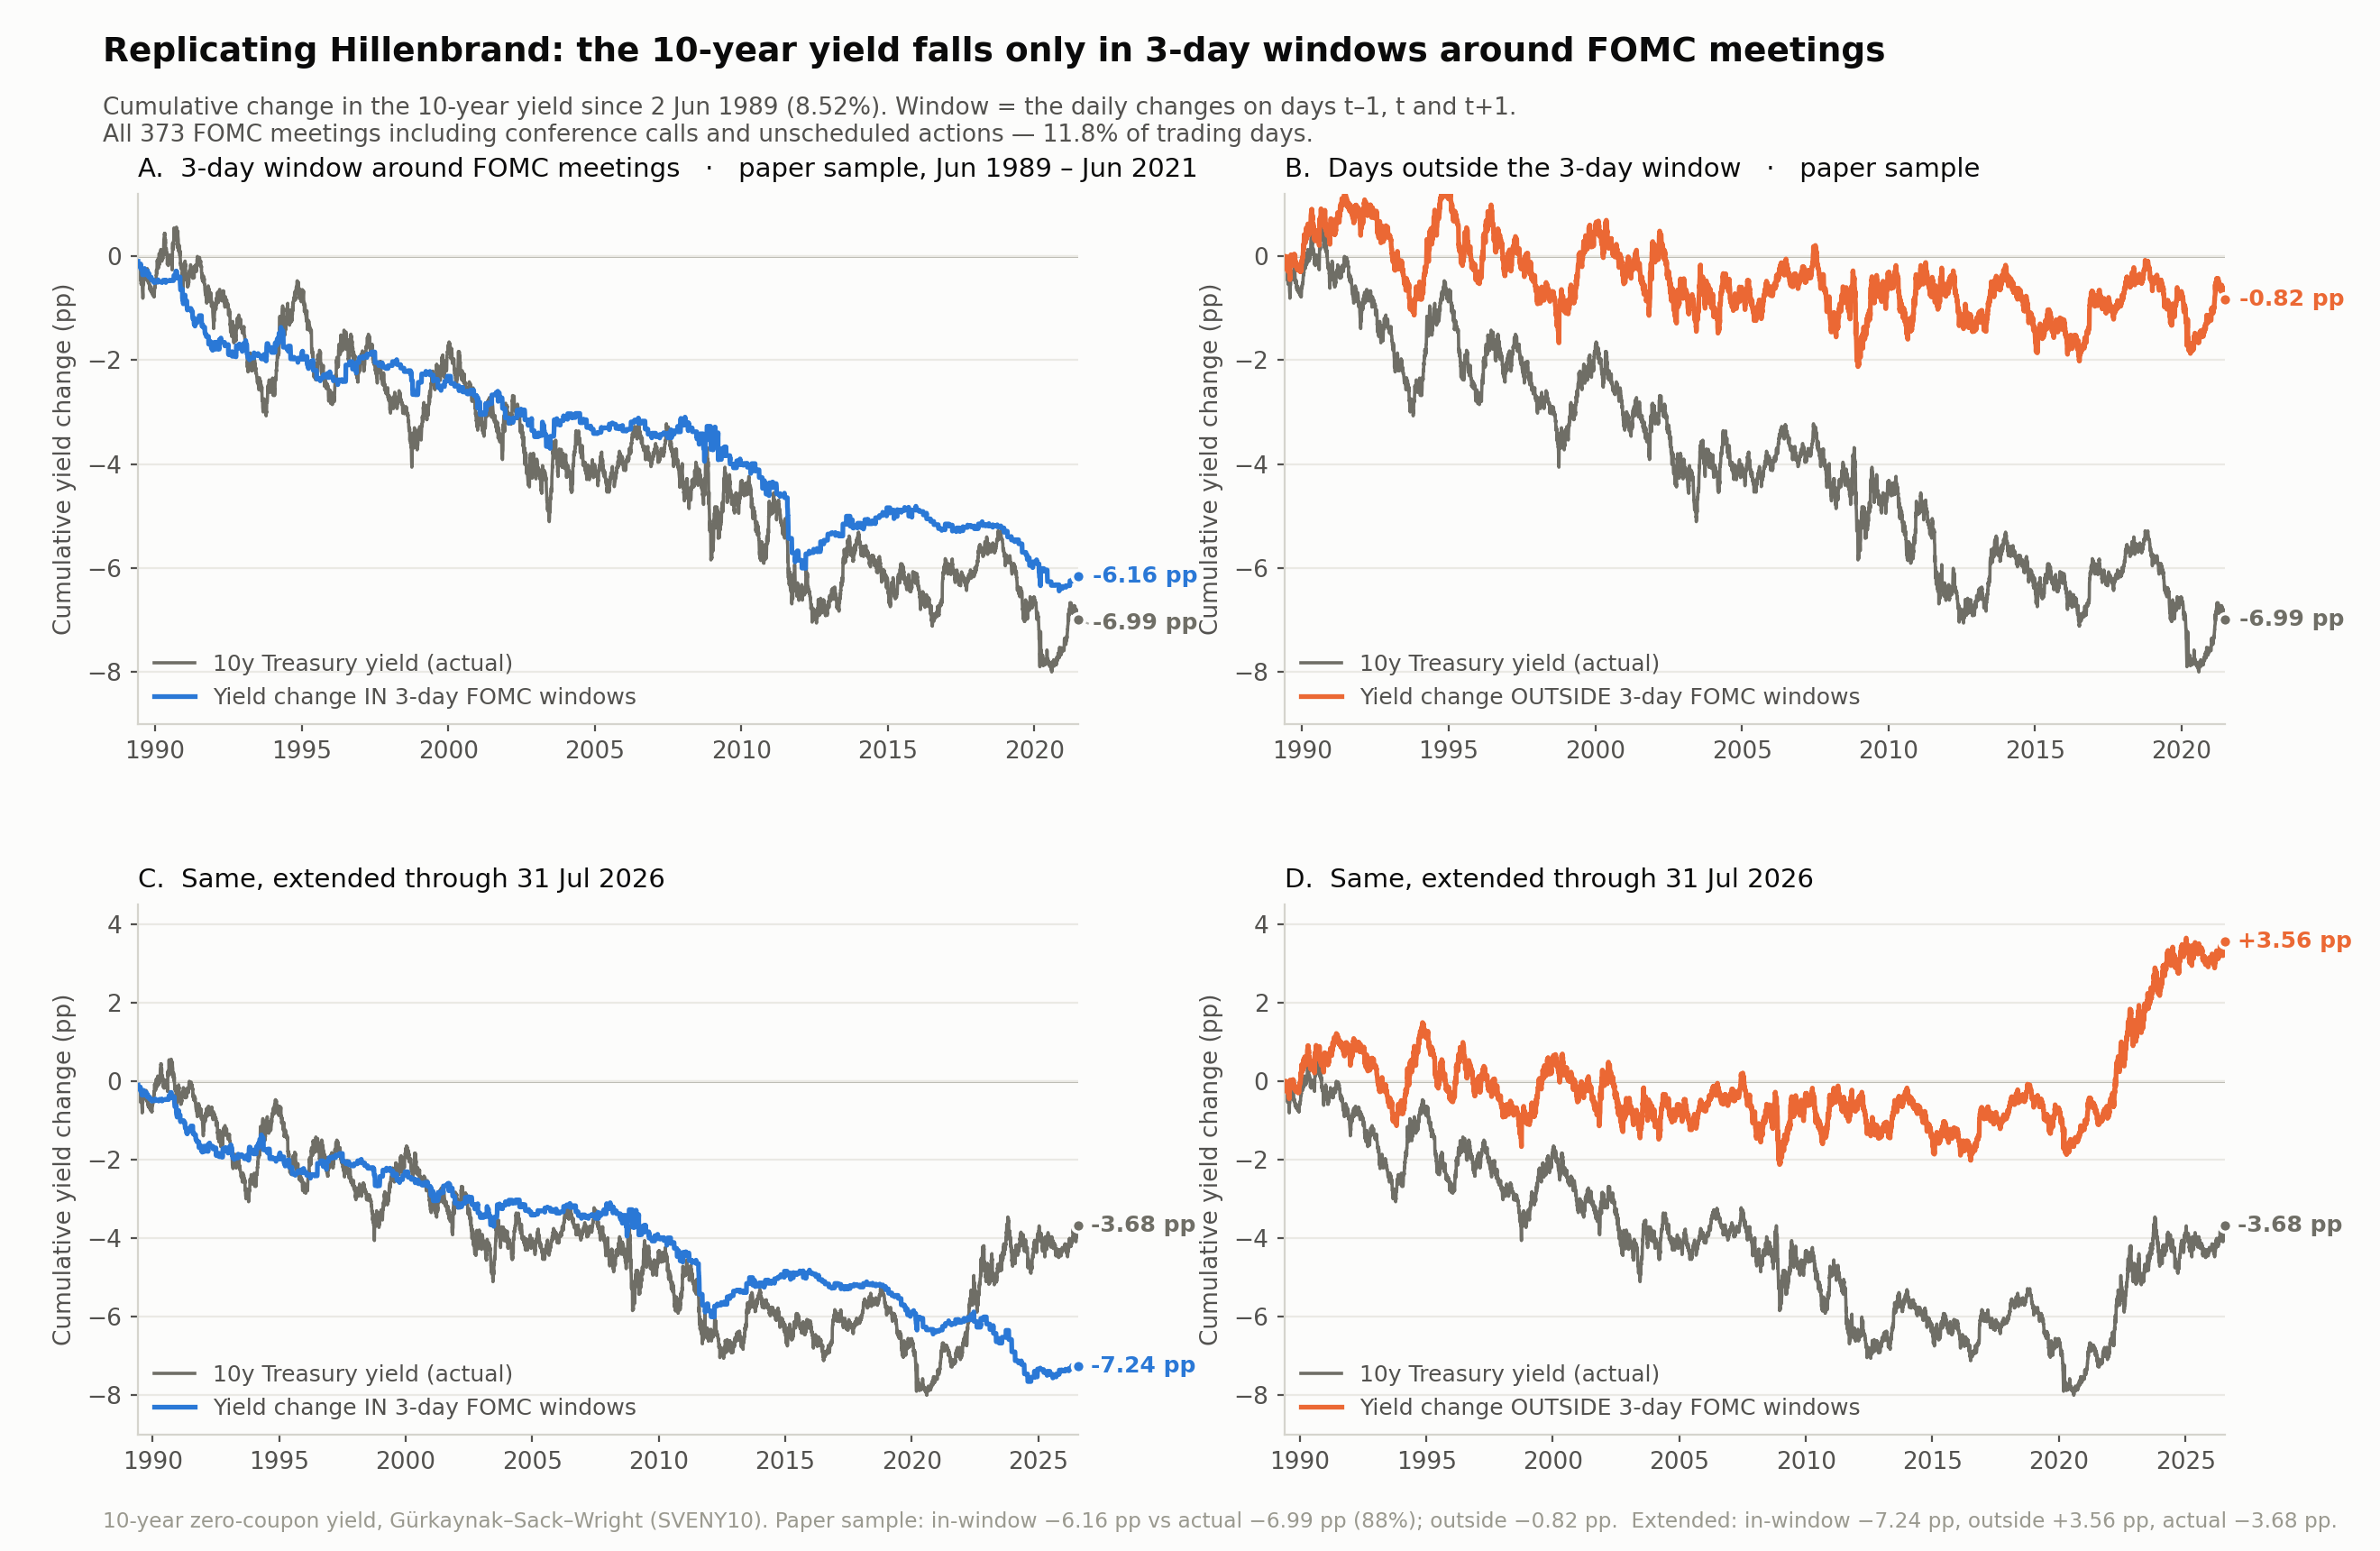
\includegraphics[width=\textwidth]{hillenbrand_paper_spec.png}
\caption{\textbf{Replication and extension.} Panels A--B reproduce the paper's sample (June 1989 -- June 2021): the 10-year yield falls 6.99 pp, 6.16 pp of it inside three-day FOMC windows and 0.82 pp outside. Panels C--D extend to 31 July 2026. The in-window series continues down to $-7.24$ pp while the outside series turns sharply positive to $+3.56$ pp --- the entire 2022--2026 tightening in long rates happened on non-FOMC days. GSW zero-coupon yields; all 373 events including conference calls and unscheduled actions (11.8\% of trading days).}
\label{fig:replication}
\end{figure}

\noindent The natural question --- and the one the literature is fighting over --- is which component of the yield moves: expected future short rates, or the term premium.

\section{Result 1: the literature's disagreement is a sample-definition artifact}

Two circulating papers give opposite answers. Hofmann, Li \& Wu (BIS WP 1252) decompose the whole window and conclude it is risk-neutral. Pan \& Peng (SSRN 4764451) decompose the pre-announcement day and conclude it is term premium.

I reproduce Pan \& Peng's estimates on their specification --- scheduled meetings only, September 1994 onward --- to three coefficients:

\begin{center}\small
\begin{tabular}{lcc}
\toprule
Day $t-1$, 10-year & Mine & Theirs\\ \midrule
Yield & $-0.785$ ($t\,{-}2.39$) & $-0.79$ ($t\,{-}2.39$)\\
Term premium & $-0.716$ ($t\,{-}2.36$) & $-0.71$ ($t\,{-}2.34$)\\
Expected short rate & $-0.070$ ($t\,{-}0.31$) & $-0.08$ ($t\,{-}0.26$)\\
\bottomrule\end{tabular}
\end{center}

\noindent and then show the attribution is not robust. The term-premium share of the day-$(t{-}1)$ decline moves from \textbf{91\%} (scheduled meetings, 1994 onward) to \textbf{46\%} (all events, 1989 onward). The mechanism is identified: the 73 conference calls and unscheduled actions that a scheduled-only filter removes contribute $-1.78$ pp of risk-neutral decline on day $t-1$ alone, about $-2.5$ bp per event against a scheduled-meeting average of $-0.07$ bp. Emergency intermeeting actions are preceded by days of expectations repricing; scheduled announcements are not.

Neither paper discusses the event list. This is a finished result requiring no model to be correct, and it is the most immediately publishable thing I have.

\section{Result 2: the standard decomposition cannot settle the question}

In a spanned affine model the state is recoverable from yields, so the expectations component is a fixed linear function of the curve: $\Delta rn^{(n)}_t=c_n'\Delta y^{\mathcal N}_t$ with $c_n'=b_n'\mathbf B^{-1}$. Regressing the daily change in the ACM 10-year risk-neutral rate on six yield changes gives $R^2=1.00000$.

The consequence for event studies is that component responses are determined by the maturity profile of the yield response: $\beta^{rn}=c'\beta^{\mathcal N}$. Applied to my estimated profile this predicts $+2.5$ and $+29.3$ bp against directly estimated $+2.6$ and $+29.2$. The decomposition adds no event-specific information; it applies historically estimated persistence weights to a profile already in hand.

Those weights are also known to be wrong for this application. Since the VAR is stationary, $b_n\to0$ and the expectations component is asymptotically constant, so genuine endpoint variation is mechanically booked as term premium. Empirically $c'\boldsymbol 1=0.529$: a permanent, credible parallel shift --- 100\% expectations by construction --- is reported as 53\% expectations and 47\% term premium.

\textit{Attribution.} The algebra is a corollary of Joslin, Singleton \& Zhu (2011) and appears as a criticism in Joslin, Priebsch \& Singleton (2014). The stationarity bias is Bauer \& Rudebusch (2020, \emph{AER}), who report 75\% versus 35--37\% for the secular decline, and Bauer \& Rudebusch (2014), who report the $\approx$50/50 event-window figure. My contribution is the explicit filter for ACM and the event-study corollary, not the theorem.

\section{Result 3: the effect and the measurement do not overlap in time}

Splitting the in-window drift by period:

\begin{center}\small
\begin{tabular}{lrrrr}
\toprule
Period & Meetings & bp/meeting & $t$ & Cumulative\\ \midrule
Jun 1989 -- Dec 2011 (pre-SEP) & 245 & $-2.46$ & $-3.06$ & $\mathbf{-5.85}$ pp\\
Jan 2012 -- Mar 2022 (dot falling $1.78$ pp) & 85 & $-0.40$ & $-0.41$ & $-0.23$ pp\\
Mar 2022 -- Jul 2026 (dot rising $0.74$ pp) & 35 & $-3.49$ & $-1.53$ & $-1.16$ pp\\
\bottomrule\end{tabular}
\end{center}
\vspace{-0.4em}
{\footnotesize\noindent Cumulative column sums daily in-window changes; days shared by adjacent events are counted once.}

\noindent Two things follow (Figure~\ref{fig:rstar}, Panel C). First, the phenomenon is overwhelmingly pre-2012, so projection-based tests are estimated where the effect is weakest. Second, during the decade when the FOMC cut its own longer-run rate by 1.78 pp --- the episode in which an information channel should be most visible --- the in-window contribution is indistinguishable from zero.

The 2022--2026 extension sharpens this. The Fed raised the target 525 bp and revised its longer-run dot \emph{up} 0.74 pp. The 10-year rose 2.60 pp. In FOMC windows it fell 1.20 pp; the entire increase occurred outside. No paper in this literature covers this period --- Hillenbrand ends June 2021, Hofmann--Li--Wu 2023, Adrian et al.\ November 2021.


\begin{figure}[tbp]
\centering
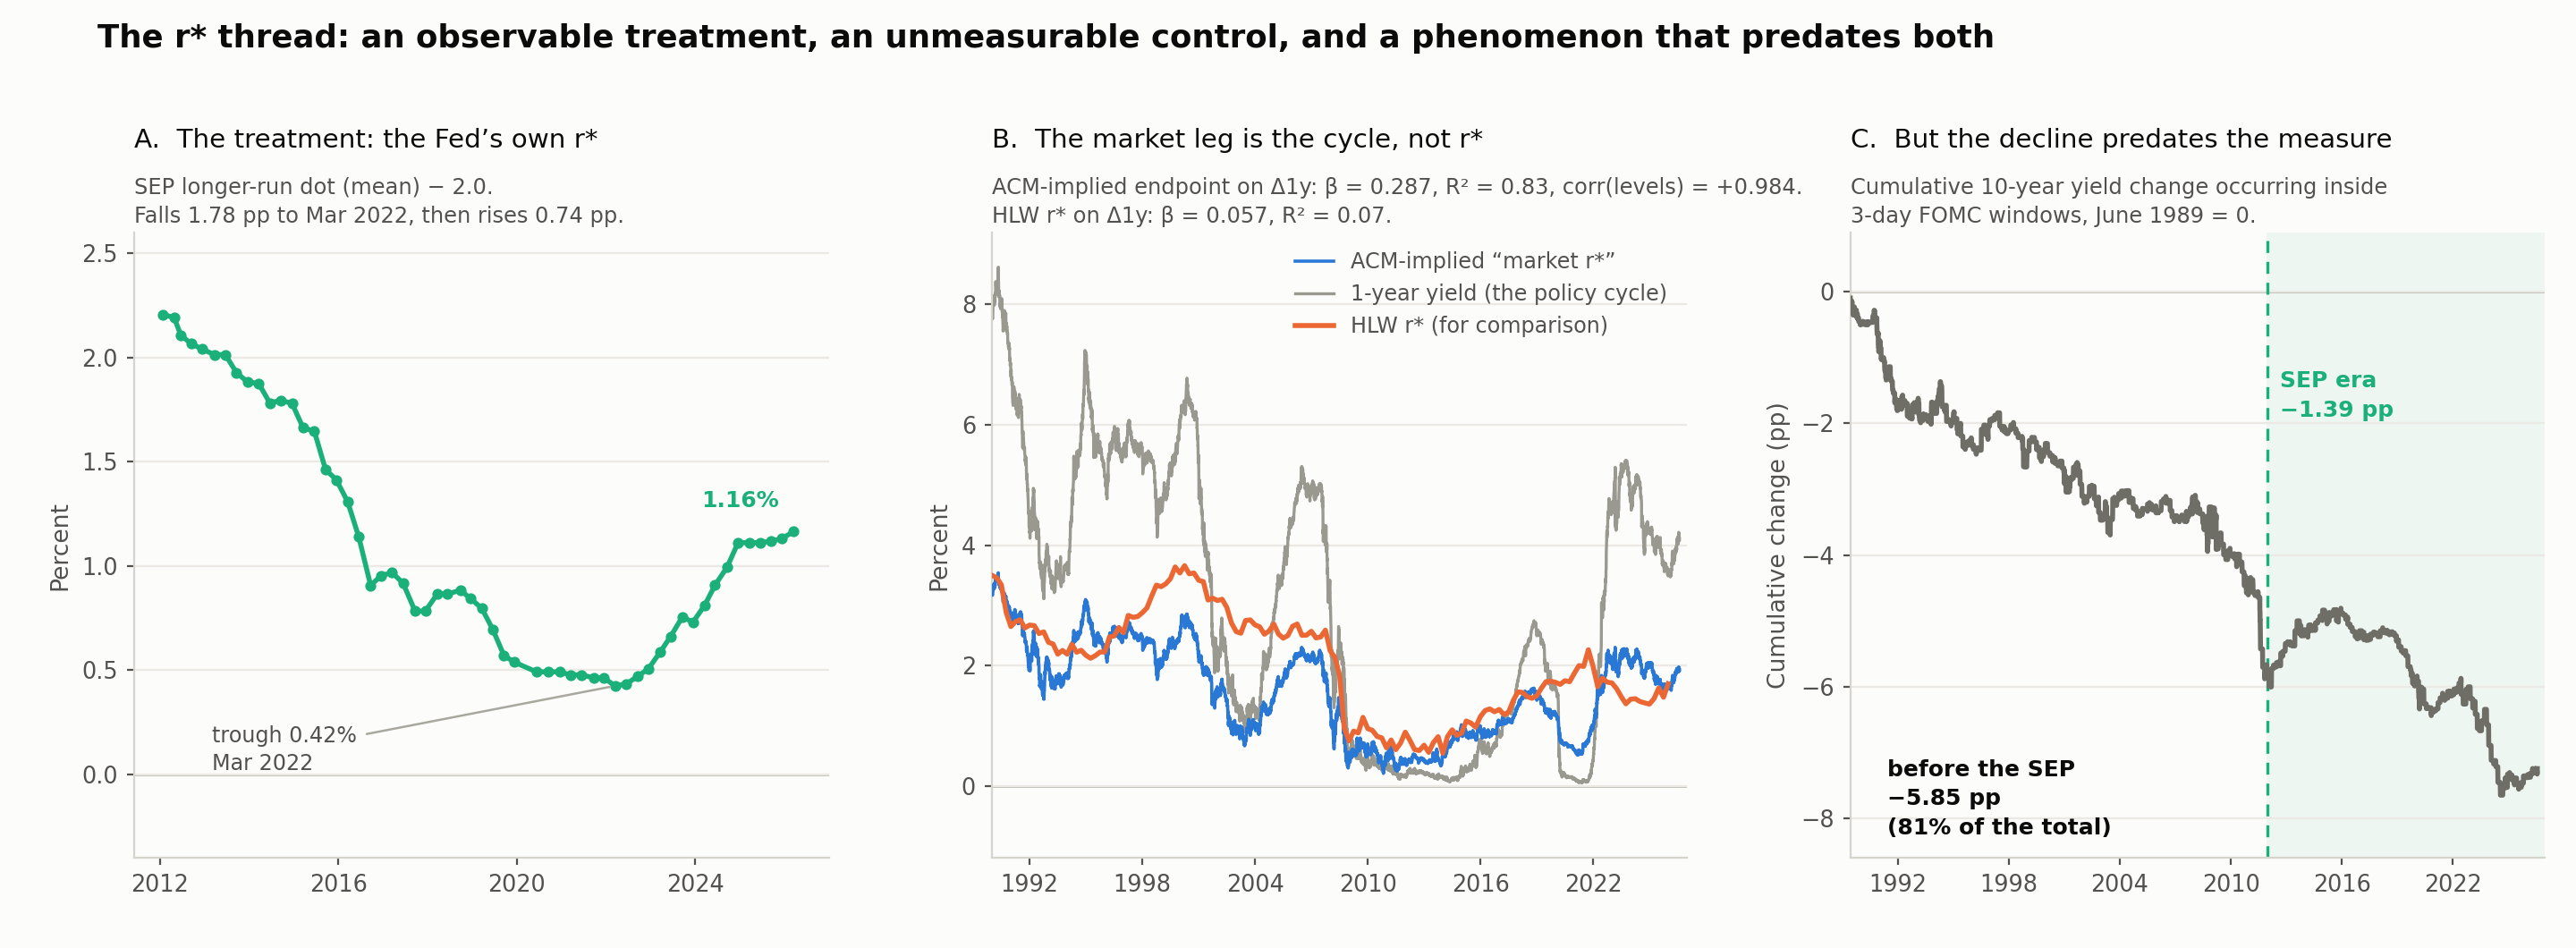
\includegraphics[width=\textwidth]{rstar_thread.png}
\caption{\textbf{Why the r\textsuperscript{*} design fails.} \emph{Panel A:} the intended treatment --- the FOMC's own longer-run real rate (SEP longer-run projection minus the 2\% target). It exists only from 2012. \emph{Panel B:} the intended market counterpart. The ACM-implied 9y1y risk-neutral forward loads on the current one-year yield with $\beta=0.287$, $R^2=0.83$ and a level correlation of $+0.984$; it is a damped copy of the policy cycle, not an endpoint estimate (HLW, by contrast, is nearly orthogonal to the cycle). \emph{Panel C:} the timing problem --- 5.85 pp of the 7.24 pp cumulative in-window decline, roughly 81\%, is complete before the dot plot begins.}
\label{fig:rstar}
\end{figure}

\section{What I have set aside, and why}

\begin{itemize}\setlength\itemsep{0.15em}
\item \textbf{The Fed--market wedge} (Figure~\ref{fig:rstar}). The market leg requires an endpoint measure. The ACM 9y1y risk-neutral forward has $\beta=0.287$ on the one-year yield with $R^2=0.83$ and a level correlation of $0.984$; it is a damped copy of the policy cycle, not an $r^{*}$ estimate. Survey alternatives correlate $-0.12$ with it and barely move.
\item \textbf{A credibility asymmetry between dovish and hawkish signals.} With 18 upward revisions I have 21--31\% power. More importantly, Hillenbrand's Table 5 and Figure 11 already split by direction, and the ratchet mechanism is Rungcharoenkitkul, Borio \& Disyatat (BIS WP 817).
\item \textbf{Expectations versus term premium as a standalone question.} Contested by the two papers above, and unidentifiable for the reason in \S3.
\end{itemize}

\section{Path forward}

\subsection*{Immediate (four weeks)}
\textbf{(a) The issuance test.} Lou, Pintér, Üslü \& Walker (BIS WP 1232) document a supply-driven pre-announcement drift in UK gilts and claim Hillenbrand's effect concentrates in FOMC windows \emph{without} long-dated Treasury issuance. If correct, the mechanism is dealer inventory rather than monetary policy. Auction dates are public; this is a few days' work and it is decisive either way.

\noindent\textbf{(b) Draft the reconciliation note} (\S2 plus the timing fact in \S4). Self-contained, model-free, and it resolves a live disagreement.

\subsection*{Medium term (one term)}
\textbf{(c) Permanent versus transitory by day type.} Window and non-window days have almost identical daily volatility (6.72 vs 5.60 bp) but wildly different cumulative outcomes ($-6.16$ vs $-0.82$ pp). The drift-to-noise ratio is roughly seventeen times higher inside the window. So the question is not which component moves, but \textbf{why only scheduled-date price changes persist.} A long-horizon variance-ratio decomposition estimated separately by day type converts this from a description into a measured object, and it requires no decomposition, no endpoint measure, and no model of the term premium --- so it survives every identification problem above.

This is the direction I think is most promising and it is the one I would build a chapter around.

\subsection*{Contingent}
\textbf{(d) Extend the Fed-side measure to the pre-2012 period}, where the effect actually lives, using Tealbook/Greenbook projections (available 1981--2019 with the five-year lag). This is the only way to test any projection-based mechanism on the sample that contains the phenomenon.

\section{Where I would value guidance}

\begin{enumerate}\setlength\itemsep{0.15em}
\item Whether the reconciliation is better as a standalone short submission or folded into a chapter as a methodological section.
\item Access to Blue Chip Financial Forecasts long-range and to the Tealbook archive --- both are binding constraints on (d).
\item Whether the permanent/transitory framing in (c) is the right way to pose the question, or whether it is too descriptive to carry a chapter without a mechanism.
\end{enumerate}

\vspace{0.8em}
\noindent\rule{\textwidth}{0.4pt}\\[0.3em]
\footnotesize\textbf{Data.} G\"urkaynak--Sack--Wright zero-coupon yields; Adrian--Crump--Moench daily decomposition, June 1989 -- August 2026; FOMC calendar assembled from Federal Reserve historical meeting pages (300 scheduled meetings 1989--2026 plus 73 conference calls and unscheduled actions); SEP dot-plot archive, 57 meetings, January 2012 -- March 2026. All estimates recomputed from source; nothing taken from a prior write-up.
\end{document}
